\documentclass[a4paper,11pt]{article}
\usepackage{amsmath}

\usepackage[utf8]{inputenc}
\usepackage{pgfplots}
\pgfplotsset{compat=1.17}
\usepackage{graphicx}
\usepackage{float}
\usepackage{graphicx}
\usepackage{caption}
\usepackage{subcaption}
\usepackage[utf8]{inputenc}
\usepackage{amsmath}
\usepackage{amssymb}
\usepackage{enumitem}
\usepackage{lipsum}

\usepackage{hyperref}

\usepackage{pgfplots}
\pgfplotsset{compat=1.18} 

\usepackage{minted}

\begin{document}

\title{
    \textbf{Assignment 5 Report - Distributed Computing with Message Passing}
}
\author{Dean Tsankov, Kacper Lisik}
\date{\today}

\maketitle

\section*{Introduction}

In this assignment, we learn how to program and use message passing in a distributed application, as well as to program, build, and execute distributed programs in C with the MPI library.

\section*{Problem 1 - Distributed Pairing 1 (a client-server application)}

\subsection*{Task description}

\begin{minted}[
frame=single,
framesep=2mm,
baselinestretch=1.2,
fontsize=\footnotesize,
breaklines,
]{text}
Assume that a class has n students numbered 1 to n and one teacher. The teacher wants to assign the students to groups of two for a project. The teacher does so by having every student submit a request for a partner. The teacher takes the first two requests, forms a group from those students, and lets each student know their partner. The teacher then takes the following two requests, forms a second group, and so on. If n is odd, the last student "partners" with themself.

\end{minted}


\subsection*{Key points of solution}

The solution consists of creating two types of processes and allowing them to communicate asynchronously using massage passing. The teaher process simply iterates through the number of students and waits to receive a request from any of them, not particularly in order of rank by utilising the {\tt MPI\textunderscore ANY \textunderscore SOURCE} wildcard in its source parameter field. It then keeps track of how many students have been unpaired and if that number reaches 2 we now that we can pair the last two unpaired students by sending them a message including the respective other student's rank as on argument. Later there is one more check wether there was a single student left without a partner (when the total number of students is odd) we pair that one with itself. Finaly we send a massage to all students that the teacher is done and that signals each of them to share who they were paired with. This is done since in the problem instructions we are told to do the final printout after the program is done not while the allocation is happening, which is also an option.

Here is the code for the teacher function:

\begin{minted}[
frame=single,
framesep=2mm,
baselinestretch=1.2,
fontsize=\footnotesize,
breaklines,
]{c}
    (...)
    void teacher(int stNum)
    {
        int i;
        int students[stNum];
        MPI_Status status;
        int unpaired = 0; // increment when a message is recieved and if it gets to two then pair the current student with the previous one
    
        for (i = 0; i < stNum; i++)
        {
            //receive message from any source since we do not know which student will request first
            MPI_Recv(&students[i], 1, MPI_INT, MPI_ANY_SOURCE, 0, MPI_COMM_WORLD, &status);
            printf("Received request from %d\n", students[i]);
            unpaired++;
            printf("Curently unpaired %d\n", unpaired);
            if (unpaired == 2)
            {
                MPI_Send(&students[i], 1, MPI_INT, students[i - 1], 0, MPI_COMM_WORLD);
                MPI_Send(&students[i - 1], 1, MPI_INT, students[i], 0, MPI_COMM_WORLD);
                unpaired = 0;
            }
        }
        //if any student was left unpaired (odd num of students) => pair by itself
        if(unpaired == 1){
            MPI_Send(&students[stNum-1], 1, MPI_INT, students[stNum - 1], 0, MPI_COMM_WORLD);
        }
    
        for (i = 0; i < stNum;i++){
            int done = 1;
            MPI_Send(&done, 1, MPI_INT, students[i], 0, MPI_COMM_WORLD);
        }
    }
    (...)
\end{minted}

Next is the student process which is fairly simple since it essentially just sends a massage with its own rank number or id and then waits to receive a partner from the teacher process with the dedicated rank 0. Lastly in order for the printout to happen after the teacher has finished assigning pairs we wait to recieve another massage.

\begin{minted}[
frame=single,
framesep=2mm,
baselinestretch=1.2,
fontsize=\footnotesize,
breaklines,
]{c}
    (...)
    void student(int id)
    {
        int pairStId;
        MPI_Status status;
    
        //ask teacher process rank 0 for a pairing
        MPI_Send(&id, 1, MPI_INT, 0, 0, MPI_COMM_WORLD);
    
        //receive pairing from teacher
        MPI_Recv(&pairStId, 1, MPI_INT, 0, 0, MPI_COMM_WORLD, &status);
    
        //wait for teacher to pair evryone before printing
        int teacherDone = 0;
        MPI_Recv(&teacherDone, 1, MPI_INT, 0, 0, MPI_COMM_WORLD, &status);
    
        if(teacherDone){
            printf("The student %d was paired with the student %d\n", id, pairStId);
        }
    }
    (...)
\end{minted}

Ultimately the main method has the following simple form:

\begin{minted}[
frame=single,
framesep=2mm,
baselinestretch=1.2,
fontsize=\footnotesize,
breaklines,
]{c}
    (...)
    int main(argc, argv)
    int argc;
    char **argv;
    {
        int rank, size;
        MPI_Init(&argc, &argv);
        MPI_Comm_rank(MPI_COMM_WORLD, &rank);
        MPI_Comm_size(MPI_COMM_WORLD, &size);
        
        //the 0 rank process will be the teacher, anything else is a student
        if(!rank){
            //exclude teacher from the student pool
            teacher(size-1);
        }else{
            student(rank);
        }
    
        MPI_Finalize();
        return 0;
    }
    (...)
\end{minted}

\section*{Problem 6 - Exchanging Values}

\subsection*{Task description}

\begin{minted}[
frame=single,
framesep=2mm,
baselinestretch=1.2,
fontsize=\footnotesize,
breaklines,
]{text}
Consider the three program outlines (algorithms) in Lecture 15, slides 28-34, for exchanging values by interactive peers. Implement each algorithm in C using the MPI library or in Java using the socket API or Java RMI. You may use collective communication (or multicast in Java) where appropriate. Each program should execute a sequence of R rounds of exchanges. Your program should print a trace of the interesting events as they happen, but do not make the trace too verbose. Estimate and compare the performance of your programs. Build a plot that shows the total execution time of each program as a function of the number of processes (2, 4, 6, 8) and the number of rounds (1, 2, 3). When performing evaluation experiments, do not print a trace of events.
\end{minted}


\subsection*{Key points of solution}

The solution to the problem follows the directions explained in the lecture slides quite closely. As such the implementation consists of the three different approaches:
\begin{itemize}[noitemsep]
        \item Centralized.
        \item Circular.
        \item Symmetric.
    \end{itemize}

We will ommit pasting their code here since each of their respective code programs can be found on the assignment's github repository.

After executing the code we can visualize the outputs in the graph bellow, which follows the general tendencies we would expect even while the data might seem a bit sporadic.

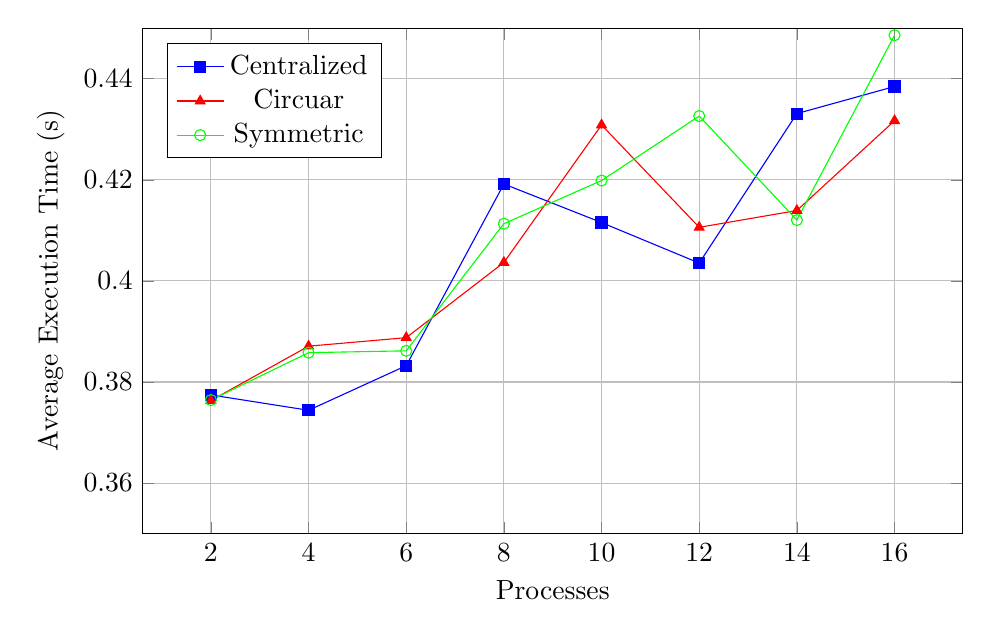
\begin{tikzpicture}
    \begin{axis}[
        width=12cm, height=8cm,
        xlabel={Processes},
        ylabel={Average Execution Time (s)},
        legend pos=north west,
        grid=major,
        xtick={2,4,6,8,10,12,14,16},
        ymin=0.35, ymax=0.45
    ]

    % Centralized data
    \addplot[color=blue, mark=square*] coordinates {
        (2,0.377441) (4,0.374404) (6,0.383231) (8,0.419178)
        (10,0.411547) (12,0.403531) (14,0.433108) (16,0.438469)
    };
    \addlegendentry{Centralized}

    % Circuar data
    \addplot[color=red, mark=triangle*] coordinates {
        (2,0.376329) (4,0.387090) (6,0.388773) (8,0.403648)
        (10,0.430855) (12,0.410604) (14,0.413928) (16,0.431700)
    };
    \addlegendentry{Circuar}

    % Symmetric data
    \addplot[color=green, mark=o] coordinates {
        (2,0.376420) (4,0.385803) (6,0.386168) (8,0.411327)
        (10,0.419862) (12,0.432619) (14,0.412046) (16,0.448612)
    };
    \addlegendentry{Symmetric}

    \end{axis}
\end{tikzpicture}


\end{document}